%=========================================================================
% (c) Michal Bidlo, Bohuslav K�ena, 2008

\chapter{GPGPU}

With high demand for real-time image processing, computer vision applications and a need for fast calculations in the scientific world, general-purpose computing on graphics processor units, also known as the GPGPU, has become a popular programming model to accelerate programs traditionally coded on the CPU (Central Processing Unit) using the data-parallel processing powers of the GPU.

Until the last decade or so, when technologies for GPGPU became available, the GPU was used mostly to render data given to it by the CPU. This has changed in a way, that the GPU, with its massive parallel capabilities, isn't used only for displaying, but also for computation. The traditional approach is to transfer data bidirectionally between the CPU and the GPU, which on one hand brings the overhead of copying the data, but on the other enables to do the calculations many times faster due to the architecture of the GPU. As shown on \ref{fig:cpu-gpu} many more transistors are dedicated to data processing instead of cache or control, which leads to a higher memory bandwidth.

\begin{center}
\begin{figure}[h]
	\centering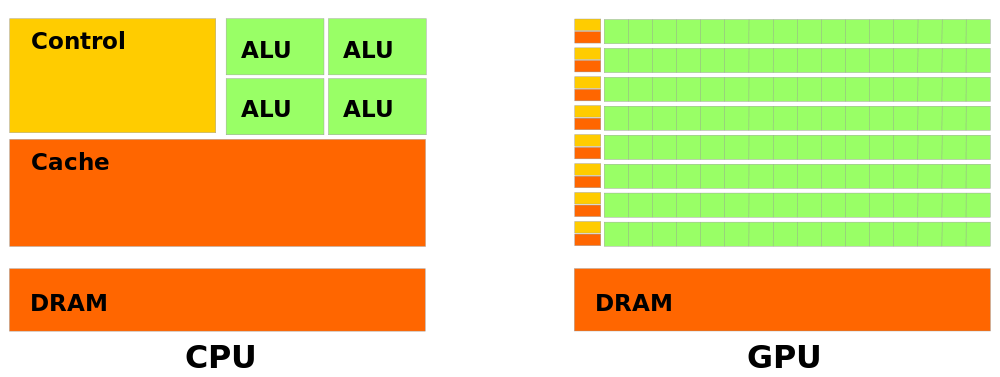
\includegraphics[height=5cm]{fig/cpu-gpu.png}
	\caption{CPU and GPU architecture comparison (\cite{cuda-toolkit-docs})}
	\label{fig:cpu-gpu}
\end{figure}
\end{center}

GPUs are also designed with demand for floating-point capabilities in mind, which can be taken advantage of in applications such as object detection, where most of the math is done in single-point arithmetic.

\begin{center}
\begin{figure}[h]
	\centering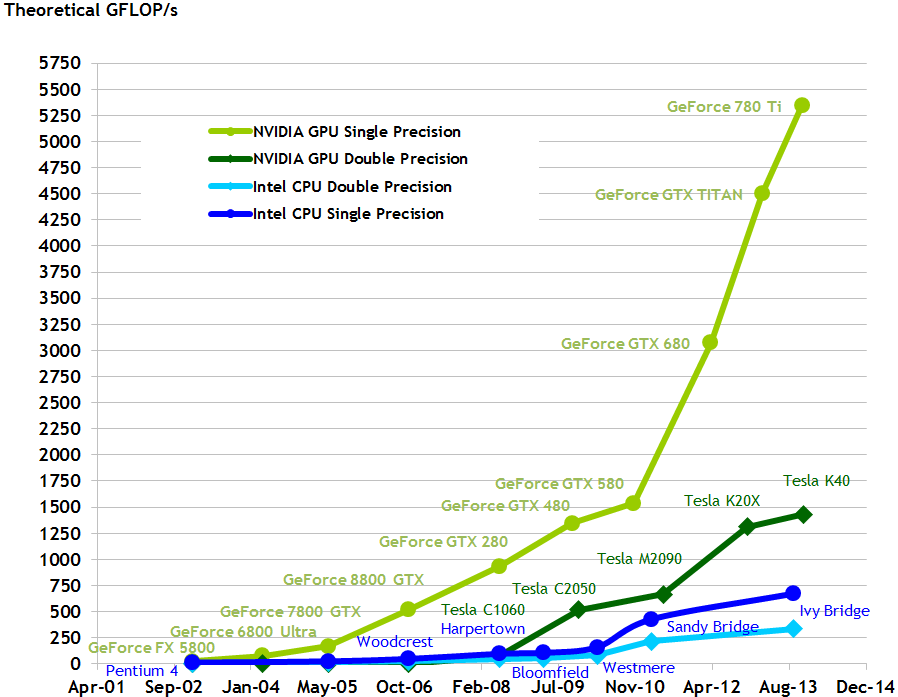
\includegraphics[height=10cm]{fig/floating-point-operations-per-second.png}
	\caption{Floating-Point operations per second for the CPU and GPU (\cite{cuda-toolkit-docs})}
\end{figure}
\end{center}

\section{Parallel computing platforms}

In November 2006 the first parallel computing platform - CUDA (Compute Unified Device Architecture) was introduced by NVIDIA. Since then several others were created by other vendors:

\begin{itemize}
	\item CUDA - NVIDIA
	\item OpenCL - Khronos Group
	\item C++ AMP - Microsoft	
	\item Compute shaders - OpenGL
	\item DirectCompute - Microsoft
\end{itemize}

All of the technologies above allow access to the GPU computing capabilities. The first two - CUDA and OpenCL work on a kernel basis. As a programmer you have access to low-level GPU capabilities and have to manage all the resources yourself. The standard approach is the following:

\begin{enumerate}
	\item Allocate memory on the GPU
	\item Copy data from the CPU to the allocated memory on the GPU
	\item Run a GPU based kernel (written in CUDA or OpenCL)
	\item Copy processed data back from the GPU to the CPU
\end{enumerate}

C++ AMP is a more higher-level oriented library. Introduced by Microsoft as a new C++ feature for Visual Studio 2012 with STL-like syntax, it is designed to accelerate code using massive parallelism. Currently it is supported by most GPUs, which have a DirectX 11 driver.

The last two - Compute shaders and DirectCompute also work in a more high-level fashion, but also quite differently from C++ AMP. They are not a part of the rendering pipeline, but can be set to be executed among other OpenGL or DirectX shaders. The difference between compute shaders and other shaders is, that they don't have specified input or output. These must be specified by the programmer. Theoretically it is then possible to write the whole rendering pipeline using compute shaders only.

\section{NVIDIA CUDA}

NVIDIA CUDA is a programming model enabling direct access to the instruction set and memory of NVIDIA GPUs.

\subsection{Programming model}

CUDA C extends C and uses NVCC compiler to generate code for the GPU. It also allows to write C-like functions called kernels. A kernel is defined by the \verb|__global__| declaration specifier and executed using a given configuration wrapped in \verb|<<< ... >>>|. The configuration is called a grid and takes as parameters the number of blocks and the number of threads. The same kernel code is run by the whole grid. Also code run by the kernel is called to device code, where as the code run outside of the kernel is called the host code.

\paragraph{Threads} are a basic computational unit identified by a 3-dimensional id \verb|threadIdx|, which is typically used to index arrays.

\paragraph{Blocks} are groups of threads, where each block resides on a single processor core, therefore a kernel can be run with the maximum of 1024 threads.

\begin{center}
\begin{figure}[h]
	\centering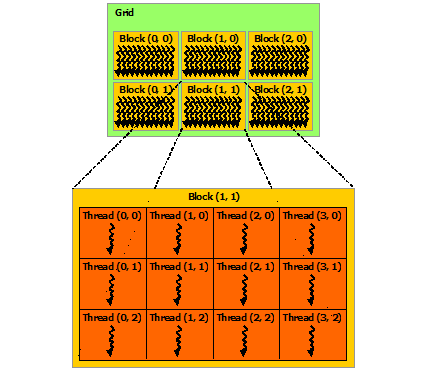
\includegraphics[height=5.5cm]{fig/grid-of-thread-blocks.png}
	\caption{A grid of blocks and threads run by a kernel (\cite{cuda-toolkit-docs})}
\end{figure}
\end{center}

Kernel configuration parameters can be passed as integers or \verb|dim3| structures. \verb|dim3| specifies the number of threads or blocks in every dimension, therefore a \verb|dim3 threadsPerBlock(4,4,1)| would run a kernel with 16 threads per block, where \verb|threadIdx.x| would range between 0 and 3 and the same for \verb|threadIdx.y|.

Example \ref{code:cuda-example} shows how to add 2 arrays in parallel using N threads and 1 block.

\begin{figure}[h]
\begin{verbatim}
// Kernel definition
__global__ void VecAdd(float* A, float* B, float* C)
{
    int i = threadIdx.x;
    C[i] = A[i] + B[i];
}

int main()
{
    ...
    // Kernel invocation with N threads
    VecAdd<<<1, N>>>(A, B, C);
    ...
}
\end{verbatim}

\caption{Example of vector addition in CUDA (\cite{cuda-toolkit-docs})}
\label{code:cuda-example}
\end{figure}

\FloatBarrier
\subsection{Memory model}\label{subsec:memory}

CUDA threads may access the following types of memories:

\begin{table}
\centering
\begin{tabular}{| l | l | l | l | l |}
\hline
Memory & Keyword & Scope & Access & Lifetime \\
\hline
Registers & - & Thread & Read/Write & Kernel \\
\hline
Local memory & - & Thread & Read/Write & Kernel \\
\hline
Shared memory & \verb|__shared__| & Block & Read/Write &  Kernel \\
\hline
Global memory & \verb|__device__| & Grid & Read/Write & Application \\
\hline
Texture memory & - & Grid & Read-only & Application \\
\hline
Constant memory & \verb|__constant__| & Grid & Read-only & Application \\
\hline
\end{tabular}
\caption{Memory types}
\end{table}

\paragraph{Global memory} is accessible by all threads in a grid and allows read-write. It is also the slowest memory type. Its access is the bottleneck for most applications with access latency ranging from 400 to 800 cycles. There are several strategies for it to be fast like coalescing access with 32B, 64B, 128B transactions.

\paragraph{Texture memory} can be regarded similarly to global memory. Cache is optimized for 2D spatial access pattern and address modes or interpolation can be used at no additional cost.

\paragraph{Constant memory} is the third memory type, which can be accessed by all threads and is typically used to store constants or kernel arguments. It doesn't bring any speed-up compared to global or texture memory, but it is optimized for broadcast.

\paragraph{Shared memory} can be accessed by all threads within a block. It is much faster than the other types, but is subject to bank conflicts.

\paragraph{Unified memory} is a memory type introduced in CUDA 6.0. It enables to use the same memory addresses both in host and device code, which simplifies writing code. On the other as of spring 2014, there doesn't seem to be any hardware support \cite{unified-memory} and the unified memory performs very similar to global memory.

\paragraph{Local memory} is a part of global memory, where everything which doesn't fit into registers is stored. For devices with Compute Capability 2.x there are 32768 32-bit registers.

\begin{center}
\begin{figure}[h]
	\centering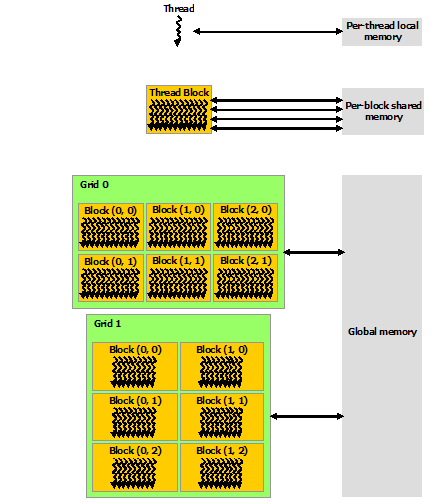
\includegraphics[height=12cm]{fig/memory-hierarchy.png}
	\caption{Memory hierarchy (\cite{cuda-toolkit-docs})}
\end{figure}
\end{center}

\chapter{Object detection}

\section{Introduction}

Object detection is a computer technology with the capability of localizing an object in  input image data. The type of object depends on which data the detector was trained. Typical applications are human faces, pedestrians, cars, traffic signs and others.

Detector used by the implementation is a frontal-face human detector, which tries to identify a human face within an image. The implementation is therefore optimized for human faces, which means, that the software can be used with other detectors, but it might effect its performance due to specific optimizations. Combined with the capabilities of a GPU, the aim is to produce an object detector capable of real-time object detection on videos.

\section{Features}

There are several methods how to access the topic of object detection. In the following sections we will discuss feature-based object detection.

Let's take a frontal human face as an example. Despite the differences such as lighting, color of eyes or skin, the length of hair, we as humans, can identify we are looking at a human face based on similarities, for example - a pair of eyes, a nose, a pair of ears and so on. These similarities can be called features, but to a computer, they are still too abstract and cannot be enumerated.

\subsection{Local Binary Pattern}

One of the feature methods to describe an image are local binary patterns (LBP). They are based on encoding local intensities of an image with 8-bit codes. In their elementary form they take a 3x3 area as an input and compare intensity values of all the pixels with the central one.

\[
 compare(p_{middle},p_{i}) =
  \begin{cases}
   1 & \text{if } p_{i} \geq p_{middle} \\
   0 & \text{else}
  \end{cases}
\]

LBP value is then evaluated as follows:

\begin{equation}
lbp(p_{middle})=\sum_{i=0}^{7} 2^{i}
compare(p_{middle},p_{i})
\end{equation}


\begin{center}
\begin{figure}[h]
	\centering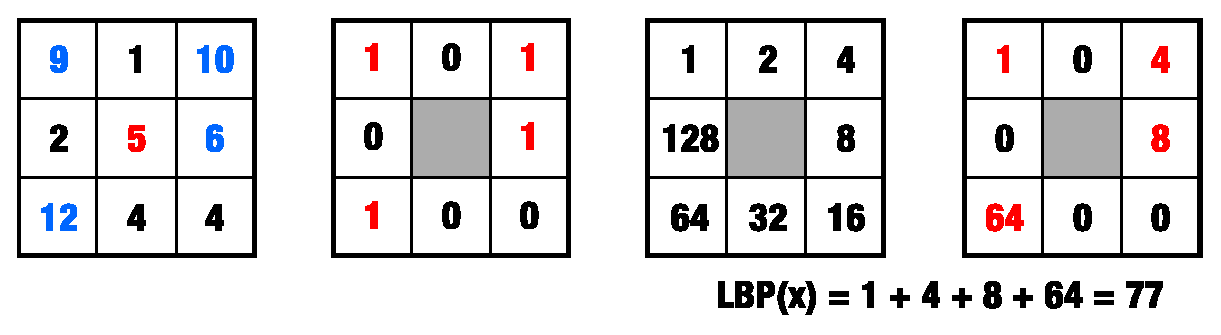
\includegraphics[width=12cm]{fig/lbp.eps}
	\caption{LBP feature}
\end{figure}
\end{center}

LBPs can be extended to be used not only for single pixels and thus 3x3 areas, but larger for larger ones. For example, when you compare 2x2 areas instead of single pixels, you compare the sum of a middle 2x2 area with the surrounding 2x2 areas.

LBP features are invariant to lighting changes, because even though the image is lighter or darker, the intensity differences stay the same. On the other hand they are not invariant to geometrical transformations such as scale or rotation.

\section{Waldboost}
\label{sec:waldboost}

Only one feature to describe a face is not enough, so a meta-algorithm to process a series of such weak classifiers is needed.

One such algorithm is WaldBoost, which combines AdaBoost and Wald's Sequential Propability Ratio Test (SPRT). SPRT is a strategy to determine what class a sample belongs to, based on a series of measurements.

\[
 SPRT =
  \begin{cases}
   +1 & \text{if } R_{m} \leq B \\
   -1 & \text{if } R_{m} \geq A \\
   \# & \text{else take another measurement} 
  \end{cases}
\]

$R_{m}$ is the likelihood ratio and A, B are constants to compute the wanted false negatives $\alpha$ and false positives $\beta$ ratios as follows:

\begin{equation}
R_{m}=\frac{p(x_{1}, ..., x_{m}|y=-1)}{p(x_{1}, ..., x_{m}|y=+1)}
\end{equation}

\begin{equation}
A=\frac{1-\beta}{\alpha}, B=\frac{\beta}{1-\alpha}
\end{equation}

As mentioned in \cite{sochman-matas-waldboost} with face detection in mind, the positive rate $\beta$ can be set to 0 and the required false negative rate $\alpha$ to a small constant. As such the equations can be simplified to

\begin{equation}
A=\frac{1-0}{\alpha}=\frac{1}{\alpha}, B=\frac{0}{1-\alpha}=0
\end{equation}

and the whole strategy to

\[
 SPRT =
  \begin{cases}
   +1 & \text{if } R_{m} \leq 0 \\
   -1 & \text{if } R_{m} \geq \frac{1}{\alpha} \\
   \# & \text{else take another measurement} 
  \end{cases}
\]

$R_{m}$ is always positive and therefore the algorithm will only classify the sample as a face when it finishes its training cycle or discard it as a background when the ratio gets greater than the given constant A.

\chapter{Implementation}

Application is implemented in \verb|C++| with dependencies on OpenCV - an open source computer vision library with \verb|C| and \verb|C++| interfaces and CUDA - a library for writing NVIDIA GPU code with a CUDA C interface, which is an extension to C. OpenCV is used to load and process separate video frames. There are also many libraries based on CUDA, which might be used in the future to enhance performance.

\begin{center}
\begin{figure}[h]
	\centering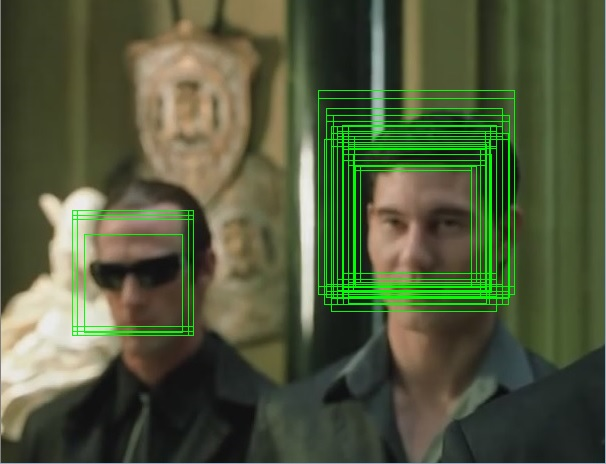
\includegraphics[height=7cm]{fig/detections.jpg}
	\caption{A sample output}
\end{figure}
\end{center}

\section{Program structure}

The basic outline of the application pipeline can be described by \ref{fig:pipeline}.

\begin{center}
\begin{figure}[h!]
	\centering\includegraphics[width=9cm]{fig/pipeline.eps}
	\caption{Application pipeline}
	\label{fig:pipeline}	
\end{figure}
\end{center}

\subsection{CUDA initialization}

In this phase all the constants and the detector itself are copied to the GPU. Constants account for data like image width and height, classifier width and height, $\alpha$ count, stage count and so on. The $\alpha$ coefficients and stages of the detector as described in \ref{sec:waldboost} are stored in separate header files generated from an XML file.

\subsection{Kernels}

After loading a video frame and copying the frame to the GPU there are 3 types of kernels to be run.

\begin{itemize}
	\item Grayscale conversion
	\item Pyramidal image build
	\item Detection
\end{itemize}

\subsubsection{Grayscale conversion kernel} \label{subsubsec:grayscale} 

Conversion to grayscale is a simple image processing operation described by the formila \eqref{eq:rgbtograyscale}. The detector itself is trained on grayscale images, and so the input must also be in grayscale. After the kernel finishes, the result is converted to a texture.

\begin{equation} \label{eq:rgbtograyscale}
Y=0.2126R + 0.7152G + 0.0722B
\end{equation}

\subsubsection{Pyramidal image kernel} 

The pyramidal image is created from the grayscale image saved in texture memory. All the features are processed inside a 26x26 pixel-wide window. The size again depends on how the detector is trained. The basic idea is that all the features inside this window somehow describe the object, so we have to create a sub-sampled image, where the object is similar or the same size as the scanning window.

As mentioned in \ref{para:grayscale} the grayscale image is stored as a texture. The advantage of this is, that it enables us to use bilinear interpolation at no performance cost. It has to be kept in mind though, that bilinear interpolation has some negative side-effects, one of them being, that sub-sampling an image below half its original size can cause errors.

\begin{center}
\begin{figure}[h]
	\centering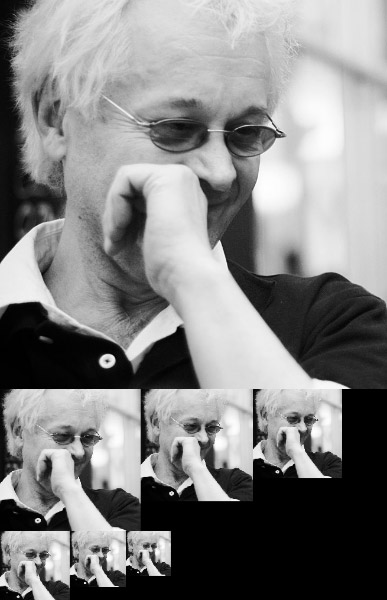
\includegraphics[height=9cm]{fig/pyramid.jpg}
	\caption{Pyramidal image}
\end{figure}
\end{center}

While the previous kernels can be viewed as preprocessing, the core of the application is the detector kernel.

\subsubsection{Detection kernel}

The detector consists of several parts, which will also be discussed later in \ref{sec:memory-organization} and how they are stored in the GPU memory.

\begin{itemize}
	\item $\alpha$ coefficient table
	\item stages
	\item final threshold
\end{itemize}

Before we discuss detection processing, let's first make clear what we mean by a stage. As mentioned in \ref{sec:waldboost} a WaldBoost algorithm processes a sample sequentially and in our case determines it is an object we are looking for only after processing all the measurements or also called stages. Every stage the algorithm processes, a response is given and added the accumulated response. If it rises above a given threshold, the sample is discarded.

Such stage is described by the following structure:

\begin{figure}[h!]
\begin{verbatim}
struct Stage {
    uint8 x, y;
    uint8 width, height;
    float thetaB;
    uint32 alphaOffset;
};
\end{verbatim}
\caption{Stage structure}
\end{figure}

The detector uses a 26x26 pixel-wide window, where \verb|x| and \verb|y| are offsets inside this window and \verb|width| and \verb|height| describe the size of the feature. Using this data, the LBP coefficient is calculated resulting in an 8-bit code. This code is then added to the \verb|alphaOffset|, which points to a specific $\alpha$, which is then added to the accumulated response. The accumulated response is then compared with \verb|thetaB| whether to discard the sample or continue processing. This can be summarized by the algorithm \ref{alg:detection}.

\begin{algorithm} \label{alg:detection}
\For{every pixel (a GPU thread is created)}
{
	\For{every stage}
	{
		1. compute LBP coefficient \\
		2. add response for the given LBP to the accumulated response \\
		\If{accumulated response $\geq$ stage threshold $thetaB$}{
			discard sample
		}
	}
}

\caption{Object detection algorithm simplified}
\end{algorithm}

\section{Memory organization} \label{sec:memory-organization}

The use of GPU memory is one of the most important parts of programming on GPU architectures. The types of CUDA memories are described in \ref{subsec:memory}.

Below we will discuss, how the most important parts of the detector are stored and why.

\begin{itemize}
\item \textbf{Stages} - constant memory \\
Stages are stored in the constant memory. Even though it's not as fast as let's say shared memory, its capability to broadcast simultaneously accessed data is ideal. Every thread processes a single image position, for which it loops through a for-cycle of stages. Every read from the constant memory is then not only broadcast to a half-warp (a group of 16 threads), but also cached. The only problem can be the size, which is limited to 64 KB. The detector uses 2048 stages, where each stage is 12 B. This leads to 24 KB, which is enough, but has to be accounted for when storing other data in the constant memory.

\item \textbf{$\alpha$ coefficients} - texture memory \\
Texture memory not only has read-only properties, but also there are 256 coefficients for every stage. Every coefficient is stored as a float, which leads to $256 * 2048 * 4 = 2 MB$ and by far exceeds the memory available for constant memory. Also the access is random, because we are likely to get different LBPs for every pixel.

\item \textbf{Original image and pyramidal image} - texture memory \\
Both are stored in the texture memory. Original image is used to create a pyramidal image using hardware accelerated bilinear interpolation for creating down-sampled images, which is a feature of the texture memory. Another feature is its read-only access.
\end{itemize}

\chapter{Results}

\section{Summary}

As of \today ~the detector contains a working GPU and CPU implementations. The CPU version is available for comparison measurements and the GPU version is unoptimized with only a few GPU acceleration features. The latest version is available at: \url{https://github.com/mmaci/vutbr-fit-object-detection}.

\begin{itemize}
	\item Memory usage is likely to stay similar, as there aren't many more viable options. The only other option is unified memory in CUDA 6.0, which seems to be more of a programmer convenient, than performance feature and shared memory, which might be used for local optimizations.
	\item Bilinear interpolation using texture memory is used for image down-sampling, instead of a software implementation.
	\item LBP for 2x1, 1x2 and 2x2 features is calculated using texture memory bilinear interpolation, which leads to a speed-up due to the fact, that sum of the intensity values isn't needed and an average is used instead.
\end{itemize}

\section{Future work}

Some of the ideas and key features yet to be implemented are:

\begin{itemize}
	\item It is generally known, that most of the samples get discarded by the WaldBoost algorithm at the beginning as background. This leads to a large number of threads waiting for the few ones, that still compute. A measurement has to be taken to statistically determine the waiting-thread count and rearrange threads in a way to increase the percentage of running threads.
	\item Other methods of interpolation, such as Lanczos interpolation should be explored and measured compared to the current bilinear interpolation.
	\item The success rate and performance of the detector is also highly dependent on the pyramid image build, therefore other ways to build an optimized pyramid should be explored or if mipmaps can be used instead and thus the whole software based interpolation omitted.
	\item The CPU version should exactly match the algorithm used for the GPU version and also be optimized to provide a valid comparison.

\end{itemize}

%=========================================================================

\nocite{zemcik-high-performance}
\nocite{herout-realtime-cuda}